\section{Controlled studies and the retrospective comparison in detail}
\label{app:controlled}
% Provenance: experiments 00, 01, 02, 06, 07, 08, 12, 13 (archived) and 14.
% make_memo_assets.py recomputes every synthetic summary below from the saved per-seed results (experiments 06, 07, 08, 13) and reads the
% retrospective rows from the committed result tables (experiments 02, 12, 14); it prints each number into assets_log.txt.

This appendix documents the synthetic studies behind Section~\ref{sec:controlled}: the data models, the judge family, the objectives, the optimizer settings and the results at every training size.
It ends with one plot of the retrospective comparison on theorem ratings.
The synthetic design of \appref{app:controlled-design} is archived experiment 13, and archived experiments 11, 12 and 14 are retrospective comparisons on theorem ratings; the archived folders keep their original numbers (\Cref{tab:index}), and the active experiment 11 is a different, later study.
\appref{app:extra-controlled} covers the other synthetic studies (experiments 01, 04, 05, 11, 15, 17 and 18).
We score every synthetic judge exactly against the known true distribution on fresh tasks.
Synthetic intervals are 95\% percentile bootstrap intervals over seeds with 10{,}000 draws and a fixed random seed.
\texttt{make\_memo\_assets.py} recomputes them from each experiment's saved per-seed results, so the last printed digit can differ from the experiment's own report.

\subsection{What each objective can learn}
\label{app:controlled-learn}

Each study fixes a model of the human ratings and asks which of its features each objective recovers (\Cref{tab:learn}).
For a one-parameter family such as $\mathrm{Bin}(5,t)$ the mean is sufficient, so a correct mean gives a correct distribution.
We assume no such family for human ratings.
Rater disagreement is extra information that only the full rating counts carry.
Proper losses use it, whereas every mean-based objective compresses those counts to one number per item, since $\E[R]=\sum_{j=0}^{K-2}\Pr[R>j]$.

\begin{table}[h]
\caption{\textbf{Mean-based objectives identify one number per item, and proper losses identify the whole distribution when the model family contains it.}
Pearson correlation identifies the conditional mean $\mu(x)$ only up to a positive affine map (Proposition~\ref{prop:affine}), and squared error identifies $\mu(x)$ exactly (Proposition~\ref{prop:losses}); the proper losses cross-entropy (CE) and ranked probability score (RPS) identify $q(\cdot\mid x)$.
Experiment 01 uses exact scoring on synthetic items and archived experiment 13 a fitted judge; experiment 02 and archived experiments 11, 12 and 14 use judges of theorem ratings without a known truth.}
\label{tab:learn}
\centering\small
\begin{tabular}{@{}p{0.085\textwidth}p{0.30\textwidth}p{0.28\textwidth}p{0.255\textwidth}@{}}
\toprule
Experiment & Human rating model & Pearson and squared error can learn & CE and RPS learn \\
\midrule
01 & $R\mid t\sim\mathrm{Bin}(5,t)$, $t\in[0.1,0.9]$; a pool of nine candidate forecasts, five of them $q_\lambda=(1-\lambda)\mathrm{Bin}(5,t)+\lambda[(1-t)\delta_0+t\delta_5]$ with $\lambda\in\{0,0.25,0.5,0.75,0.95\}$
 & $t$ only: every $q_\lambda$ has mean $5t$ (and variance $5t(1-t)(1+4\lambda)$), so these five candidates tie
 & $\lambda=0$, the truth, out of the nine: with one rating per item CE picks it in 249 of 256 draws and RPS in 245 of 256, and with two or three ratings both pick it in 256 of 256 \\
13$^{\text{a}}$ & $R\mid x\sim\mathrm{BetaBin}\bigl(5,\mu(x)\kappa(x),(1-\mu(x))\kappa(x)\bigr)$ with $\mu$ and $\kappa$ as in \appref{app:controlled-design}
 & Pearson: $\mu(x)$ up to a positive affine map. Squared error: $\mu(x)$. Neither sees $\kappa(x)$.
 & the full $q(\cdot\mid x)$, so $\mu(x)$ and $\kappa(x)$ together \\
02; 11, 12, 14$^{\text{a}}$ & $R\mid x\sim\mathrm{Cat}(p_0(x),\dots,p_5(x))$ with five unknown free probabilities per artifact
 & the mean rating only
 & the full distribution, within the judge family \\
\bottomrule
\end{tabular}

\raggedright\scriptsize$^{\text{a}}$Archived experiments keep their original numbers.
\end{table}

\subsection{Design of the synthetic study (archived experiment 13)}
\label{app:controlled-design}

\paragraph{Data model.}
A task has one feature $x\sim\mathrm{Unif}[-1,1]$ and human ratings $R\mid x\sim\mathrm{BetaBin}\bigl(5,\mu(x)\kappa(x),(1-\mu(x))\kappa(x)\bigr)$ on $\{0,\dots,5\}$.
The mean rating is $5\mu(x)$ and the variance is $5\mu(x)(1-\mu(x))(\kappa(x)+5)/(\kappa(x)+1)$.
The concentration $\kappa(x)=\exp\bigl(1.5+2.2\cos(1.5\pi x)\bigr)$ ranges from 0.50 to 40.4: small $\kappa$ splits raters toward 0 and 5, and large $\kappa$ makes them agree.
In scenario A, $\mu_A(x)=0.5+0.08x$: the true mean rating stays between 2.1 and 2.9 while the true variance ranges from 1.37 to 4.54, so almost all differences between tasks lie in the disagreement.
In scenario B, $\mu_B(x)=0.1+0.8\bigl(\tfrac{x+1}{2}\bigr)^2$: the true mean rating rises from 0.5 to 4.5, the concentration varies as in A, and the true variance ranges from 0.78 to 4.25.
The true distribution has test RPS 0.187 in scenario A and 0.136 in scenario B; RPS excess is measured from these floors.

\paragraph{Judge family and objectives.}
Every judge is the softmax-linear model $q_W(r\mid x)=\mathrm{softmax}\bigl(W^\top\phi(x)\bigr)_r$ with $\phi(x)=(1,\cos\pi x,\sin\pi x,\dots,\cos6\pi x,\sin6\pi x)\in\mathbb R^{13}$ and $W\in\mathbb R^{13\times6}$, so it has 78 weights, and its expected rating is $m_W(x)=\sum_r r\,q_W(r\mid x)$.
We train on $n$ tasks with three independent ratings each, and write $\hat p_i$, $\hat P_i$ and $\hat m_i$ for the empirical histogram, cumulative distribution function and mean of the ratings of task $i$, and $Q_W$ for the judge's cumulative distribution function.
Only the objective differs between judges:
\begin{align*}
\text{CE-trained:}\quad & \min_W\ \frac1n\sum_{i=1}^{n}\sum_{r=0}^{5}\hat p_i(r)\bigl[-\log q_W(r\mid x_i)\bigr]+\frac1n\|W\|^2,\\
\text{RPS-trained:}\quad & \min_W\ \frac1n\sum_{i=1}^{n}\frac15\sum_{j=0}^{4}\bigl(Q_W(j\mid x_i)-\hat P_i(j)\bigr)^2+\frac1n\|W\|^2,\\
\text{Pearson-trained:}\quad & \max_W\ \operatorname{corr}_{i=1,\dots,n}\bigl(m_W(x_i),\hat m_i\bigr)-\frac1n\|W\|^2 .
\end{align*}
The Pearson objective constrains only the mean $m_W(x)$, and only up to an affine map; the start and the ridge penalty set the rest of the shape.
The Pearson-trained judge with a calibrated head adds a second stage: it standardizes the Pearson-trained score $s(x)=m_W(x)$ on the training tasks, $z(x)=(s(x)-\bar s)/\mathrm{sd}(s)$, and fits a six-way softmax $q_{\mathrm{head}}(r\mid x)=\mathrm{softmax}\bigl(a_r+b_rz(x)\bigr)_r$ with $(a,b)\in\mathbb R^6\times\mathbb R^6$ by CE on the same training ratings.
This mirrors the common practice of building a scalar score and calibrating it afterwards; the head sees one number per task, so it cannot recover disagreement that the score does not carry.

\paragraph{Test metrics.}
For each seed we draw 500 fresh tasks $x'_t$ and score each judge against the true distribution $P$: RPS excess $=\frac1{500}\sum_t\frac15\sum_{j=0}^{4}\bigl(Q(j\mid x'_t)-P(j\mid x'_t)\bigr)^2$, the RPS of the forecast minus the RPS of the true distribution, and CE excess $=\frac1{500}\sum_t\mathrm{KL}\bigl(P(\cdot\mid x'_t)\,\|\,q(\cdot\mid x'_t)\bigr)$ in nats.
We floor each forecast probability at $10^{-6}$ and renormalize before scoring.
Both metrics are zero for a perfect judge, and lower is better.
We use 100 seeds at each of 11 training sizes from 4 to 2{,}048 tasks, so 12 to 6{,}144 ratings.

\paragraph{How each judge was chosen.}
We fit each judge by L-BFGS-B with analytic gradients, at most 400 iterations and 600 function evaluations, with ridge weight $1/n$.
The start reproduces the training-set marginal histogram at every $x$ (the intercept row holds its logarithm, clipped below at 0.001). It adds seeded Gaussian noise with standard deviation 0.01 to every weight. The noise breaks the tie of a constant score, for which Pearson correlation is undefined.
The softmax CE objective with ridge is convex in $W$, so its minimizer is global, but the frozen implementation clips probabilities and returns an inconsistent gradient where the clip is active, and the solver supplies no optimality certificate; a rerun with the exact objective reproduces the reported scores (\appref{app:controlled-budget}).
The RPS and correlation objectives are not convex and we have no certificate of global optimality, so every curve of a judge trained on them reflects this optimizer, start and budget.

\subsection{Learning curves: CE overtakes Pearson after twelve ratings when the mean is informative}
\label{app:controlled-curves}

\Cref{fig:exp13-curves} plots held-out test RPS excess and CE excess against training size, and \Cref{tab:exp13} lists the RPS-excess values.
In scenario B the CE-trained judge has lower RPS excess than the Pearson-trained judge at every size from 4 tasks (12 ratings), and the gap grows with size.
In scenario A the Pearson-trained judge is slightly better at 4 to 32 tasks (12 to 96 ratings), by at most 0.0027 RPS excess (at 16 tasks).
From 64 tasks (192 ratings) the CE-trained judge is significantly better at every size, on RPS excess and on CE excess.
We offer one reading of the small-sample result in A, which we did not test directly.
The Pearson-trained judge starts at the training histogram and keeps roughly that shape, a good guess when the mean barely moves, while the flexible CE-trained judge needs more ratings to learn how disagreement varies with $x$.

At 2{,}048 tasks (6{,}144 ratings) the RPS excess of the Pearson-trained judge is 36.7 times that of the CE-trained judge in scenario A (0.0251 against 0.0007) and 25.5 times in scenario B (0.0951 against 0.0037).
Its CE excess is 0.3937 nats in A and 0.5957 in B, against 0.0065 and 0.0222 for the CE-trained judge.
The RPS-trained judge matches the CE-trained judge on RPS excess (0.0009 against 0.0007 in A, 0.0038 against 0.0037 in B). It has a larger CE excess (0.0134 against 0.0065 in A, and 0.0372 against 0.0222 in B). This is consistent with RPS being less sensitive than CE to the probability of rare ratings.

\begin{figure}[t]
\centering
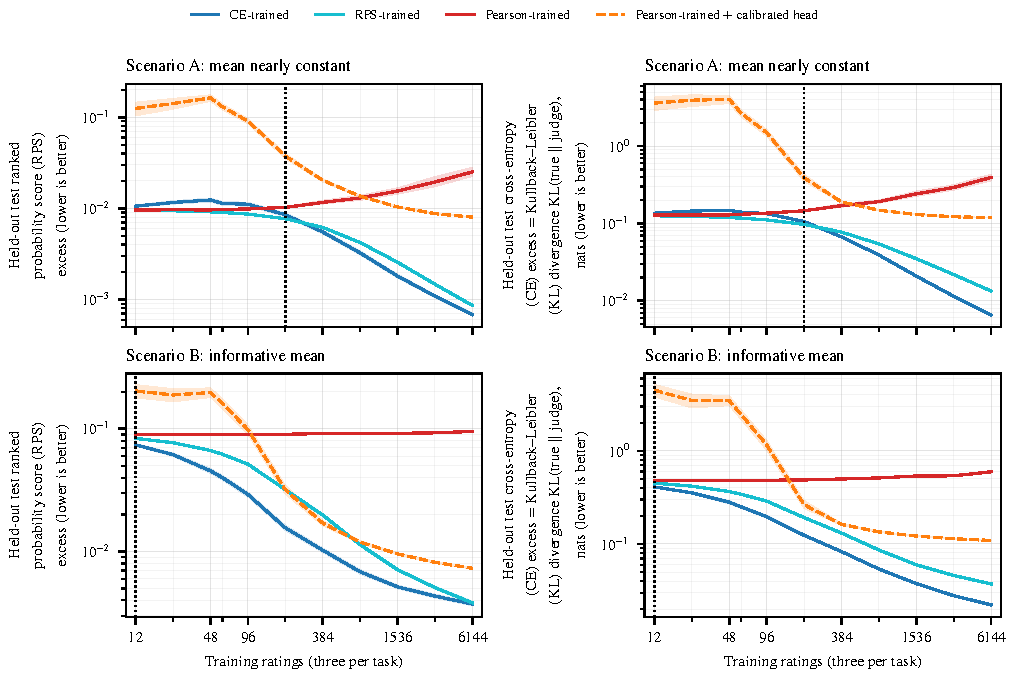
\includegraphics[width=0.96\textwidth]{figures/fig_exp13_curves.pdf}
\caption{\textbf{The CE-trained judge's error falls with more ratings, while the Pearson-trained judge's error stays flat or rises.}
Data: synthetic tasks with known rating distributions (experiment 13), 100 seeds per size, scored on 500 fresh tasks per seed.
Left column: held-out test ranked probability score (RPS) excess, the RPS of the forecast minus the RPS of the true distribution (0 is best; lower is better; log scale).
Right column: held-out test CE excess, $\mathrm{KL}(\text{true}\,\|\,\text{judge})$ in nats (0 is best; lower is better; log scale).
Horizontal axis: training ratings, three per task.
Rows: scenario A (nearly constant mean) and B (informative mean).
We chose each judge by L-BFGS-B (at most 400 iterations) from the training-histogram start with ridge weight $1/n$.
The CE objective is convex and the RPS and Pearson objectives are not, so their curves reflect this optimizer, start and budget.
Bands: 95\% percentile bootstrap intervals over seeds (10{,}000 draws).
Dotted vertical line: the smallest training size from which the CE-trained judge is significantly better than the Pearson-trained judge at every larger size (paired 95\% bootstrap lower bound above 0).}
\label{fig:exp13-curves}
\end{figure}

\begin{table}[t]
\caption{\textbf{The cross-entropy (CE)-trained judge's advantage grows with data in both scenarios, and is negative only in scenario A below 64 tasks.}
Held-out test ranked probability score (RPS) excess (0 is best; lower is better), mean over 100 seeds on 500 fresh tasks per seed.
The difference columns give the test RPS excess of the Pearson-trained judge minus that of the CE-trained judge, paired by seed, with a 95\% percentile bootstrap interval over seeds (10{,}000 draws); positive means the CE-trained judge is better.
We chose the judges as in \Cref{fig:exp13-curves}.}
\label{tab:exp13}
\centering\scriptsize
\setlength{\tabcolsep}{3pt}
\begin{tabular}{@{}rrrrrrr@{}}
\toprule
 & \multicolumn{3}{c}{Scenario A (mean nearly constant)} & \multicolumn{3}{c}{Scenario B (informative mean)} \\
\cmidrule(lr){2-4}\cmidrule(lr){5-7}
Tasks (ratings) & CE & Pearson & Pearson $-$ CE [95\% CI] & CE & Pearson & Pearson $-$ CE [95\% CI] \\
\midrule
4 (12) & 0.0106 & 0.0096 & -0.0010 [-0.0013, -0.0006] & 0.0740 & 0.0901 & +0.0161 [+0.0145, +0.0178] \\
8 (24) & 0.0116 & 0.0096 & -0.0020 [-0.0025, -0.0015] & 0.0616 & 0.0897 & +0.0281 [+0.0261, +0.0302] \\
16 (48) & 0.0123 & 0.0096 & -0.0027 [-0.0034, -0.0021] & 0.0454 & 0.0898 & +0.0444 [+0.0423, +0.0466] \\
32 (96) & 0.0111 & 0.0098 & -0.0013 [-0.0019, -0.0007] & 0.0292 & 0.0897 & +0.0606 [+0.0591, +0.0621] \\
64 (192) & 0.0085 & 0.0102 & +0.0017 [+0.0012, +0.0022] & 0.0156 & 0.0902 & +0.0747 [+0.0736, +0.0756] \\
128 (384) & 0.0055 & 0.0116 & +0.0061 [+0.0055, +0.0069] & 0.0102 & 0.0915 & +0.0813 [+0.0805, +0.0821] \\
2048 (6,144) & 0.0007 & 0.0251 & +0.0244 [+0.0217, +0.0277] & 0.0037 & 0.0951 & +0.0914 [+0.0894, +0.0936] \\
\bottomrule
\end{tabular}

\end{table}

\paragraph{A calibrated head does not close the gap.}
The Pearson-trained judge followed by a calibrated head never beats the CE-trained judge: its mean RPS excess is lower at none of the tested sizes.
It is far worse at small sizes, with RPS excess 0.1248 at 4 tasks in scenario A against 0.0106 for the CE-trained judge, and 0.2034 against 0.0740 in B.
The head beats the raw Pearson-trained judge (paired lower bound above 0 at every larger size) from 512 tasks (1{,}536 ratings) in A and from 64 tasks (192 ratings) in B.
At 2{,}048 tasks its RPS excess is 0.0080 in A and 0.0073 in B, against 0.0007 and 0.0037 for the CE-trained judge.
\Cref{fig:exp13-dist} shows why: where the mean is almost constant, the Pearson score barely varies, and one calibrated number cannot carry spread that it does not hold.
At $x=-0.7$ the raters split, and the true probability of the two extreme ratings is 0.66; the CE-trained judge assigns 0.62 and the calibrated head 0.34.
At $x=0$ the raters agree (0.08 on the extremes; CE-trained 0.07), and at $x=0.5$ they split again (0.51; CE-trained 0.53), yet the head assigns 0.34 at all three values.
The total variation distance to the true distribution is 0.07, 0.04 and 0.05 for the CE-trained judge against 0.32, 0.26 and 0.18 for the calibrated head.

\begin{figure}[t]
\centering
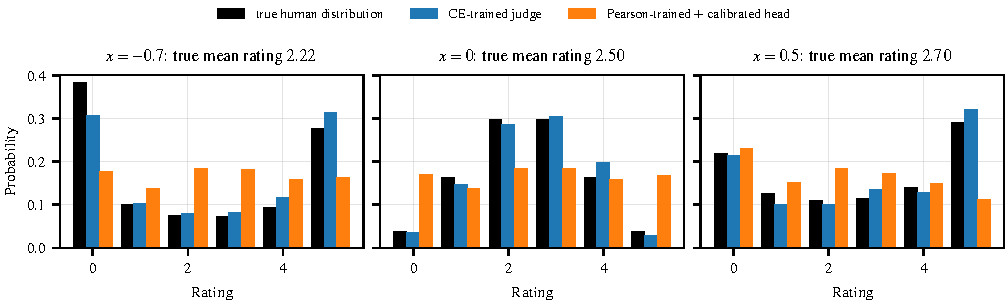
\includegraphics[width=0.96\textwidth]{figures/fig_exp13_distributions.pdf}
\caption{\textbf{The CE-trained judge recovers the split between ratings 0 and 5, and the calibrated Pearson score cannot.}
Data: scenario A of experiment 13 with 1{,}024 training tasks and three ratings per task, one illustrative training set drawn with a fixed random seed by \texttt{make\_memo\_assets.py} using experiment 13's code (not one of the 100 saved seeds).
Each panel shows one value of $x$ with a similar true mean rating (2.22, 2.50 and 2.70): black bars are the true human rating distribution, blue bars the CE-trained judge and orange bars the Pearson-trained judge with a calibrated head.
Vertical axis: probability of each rating.
We chose each judge by L-BFGS-B from the training-histogram start.
The CE objective is convex and the Pearson objective is not, so the orange bars reflect this optimizer, start and budget.}
\label{fig:exp13-dist}
\end{figure}

\paragraph{High correlation with a large distributional error, even without sampling noise.}
We also fit each objective on a dense 4{,}000-point grid of true distributions with near-zero ridge and the same optimizer and start, which removes sampling noise.
The same grid scores every fit, so each value in this paragraph is an in-sample numerical reference, not a held-out result or a proven large-sample limit, and the correlation fits are not certified optimal.
On the grid the Pearson-trained judge reaches Pearson correlation 0.9987 with the true mean in scenario A and 0.9988 in B, and its RPS excess is still 0.0872 and 0.0281.
The CE-trained judge has lower correlation (0.9395 and 0.9704) and far lower RPS excess (0.0003 and 0.0035).
With a calibrated head the Pearson-trained judge's RPS excess falls to 0.0072 and 0.0057 (correlation 0.9987 and 0.9946), which is still above the CE-trained judge's in both scenarios.

\subsection{Rank correlations and a Pearson--Spearman mix do not change the picture (experiment 06)}
\label{app:controlled-rank}

Experiment 06 trains the same 78-weight judge on the identical tasks, seeds and test tasks as experiment 13, with three further objectives. These are the Spearman correlation, Kendall's $\tau$ and the average of the Pearson and Spearman correlations between the judge's expected rating and the training-task mean ratings.
Rank correlations are not differentiable, so training uses smooth surrogates with temperature 0.1 rating points.
Refitting the CE-trained judge on the regenerated tasks (seed 0 in each of 22 scenario-by-size cells) reproduces experiment 13's saved RPS excess to within 7.6e-15.

In scenario B the CE-trained judge beats all four correlation-trained judges on test RPS excess from 4 tasks (12 ratings).
In scenario A it beats the Kendall-trained judge from 8 tasks (24 ratings) and the Pearson-trained, Spearman-trained and half-and-half judges from 64 tasks (192 ratings).
At 2{,}048 tasks the RPS excess of the correlation-trained judges is 8.8 to 25.5 times that of the CE-trained judge in B (0.0330 to 0.0951 against 0.0037) and 36.5 to 45.8 times in A (0.0249 to 0.0313 against 0.0007).
The half-and-half objective stays close to Pearson alone, so the tested equal-weight mix does not remove the distributional error (we did not test other weights), and the Kendall-trained judge has the largest RPS excess in A.

\begin{figure}[t]
\centering
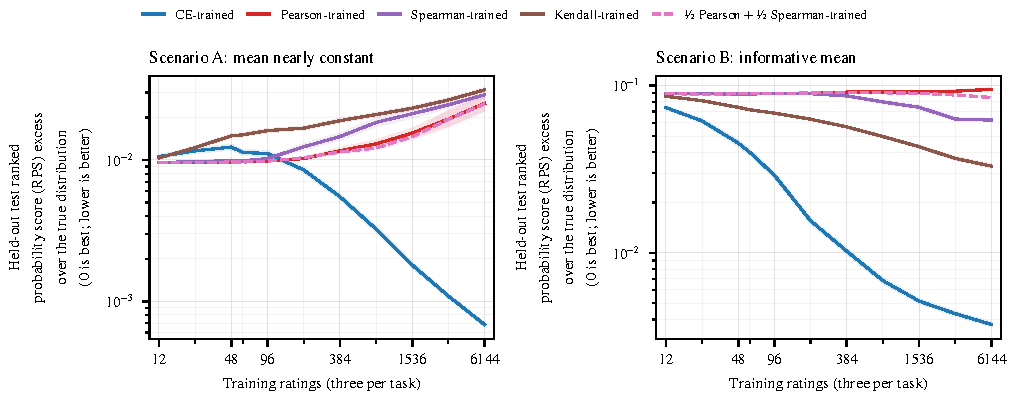
\includegraphics[width=0.96\textwidth]{figures/fig_exp06_rank.pdf}
\caption{\textbf{No tested correlation objective reaches the cross-entropy (CE)-trained judge's ranked probability score (RPS) excess, and in scenario A the rank objectives are worse than Pearson.}
Data: synthetic tasks with known distributions (experiments 06 and 13; identical training and test tasks), 100 seeds per size, 500 fresh test tasks per seed.
Vertical axis: held-out test RPS excess over the true distribution (0 is best; lower is better; log scale); horizontal axis: training ratings, three per task.
We chose each judge by L-BFGS-B (at most 400 iterations) from the training-histogram start with ridge weight $1/n$; rank objectives use smooth surrogates (temperature 0.1).
None of the correlation objectives is convex and we certified no fit, so these curves reflect this optimizer, start and budget.
Bands: 95\% percentile bootstrap intervals over seeds (10{,}000 draws).}
\label{fig:exp06-rank}
\end{figure}

\paragraph{Even on correlation, training on correlation buys little.}
In scenario A no correlation-trained judge has a higher mean test correlation than the CE-trained judge at any tested size, measured by Pearson correlation for the Pearson-trained and half-and-half judges and by Spearman correlation for the Spearman-trained and Kendall-trained judges (we did not evaluate Kendall's $\tau$ itself). At 2{,}048 tasks the CE-trained judge's test Pearson correlation with the true mean is 0.89, against 0.75 to 0.85 for the correlation-trained judges.
In scenario B the lead is just as wide at small sizes: at 16 tasks (48 ratings) the CE-trained judge's test Pearson correlation is 0.69, against 0.09 to 0.57 for the four correlation-trained judges.
The correlation-trained judges overtake on that correlation only with plenty of data.
In scenario B none has a higher mean correlation below 128 tasks.
In scenario B the differences become significant (paired lower bound above 0 at every larger size) from 256 tasks (768 ratings) for the Spearman-trained and Kendall-trained judges on test Spearman correlation, and from 512 tasks (1{,}536 ratings) for the Pearson-trained and half-and-half judges on test Pearson correlation.
In scenario B at 2{,}048 tasks the Spearman-trained judge's test Spearman correlation is 0.982 against 0.948 for the CE-trained judge, yet its RPS excess is 16.7 times as large.
A likely reason for the small-sample gap, which we did not test, is that the CE-trained judge learns from every rating, while a correlation-trained judge sees one noisy mean per task.

\subsection{The crossovers survive larger optimizer budgets and restarts (experiment 07)}
\label{app:controlled-budget}

Experiments 13 and 06 fit each judge once from one start, and the correlation objectives are not convex.
Experiment 07 reruns the same tasks (30 seeds, 4 to 1{,}024 training tasks) under three conditions.
The first is the original setting.
The second keeps the original start and raises the budget to 2{,}000 iterations and 4{,}000 function evaluations.
The third takes the best of five starts at that budget, chosen by the penalized training objective, so test data never enter the choice.
The CE reference has one start per budget, and we refit each calibrated head once on the selected Pearson score.

\begin{figure}[t]
\centering
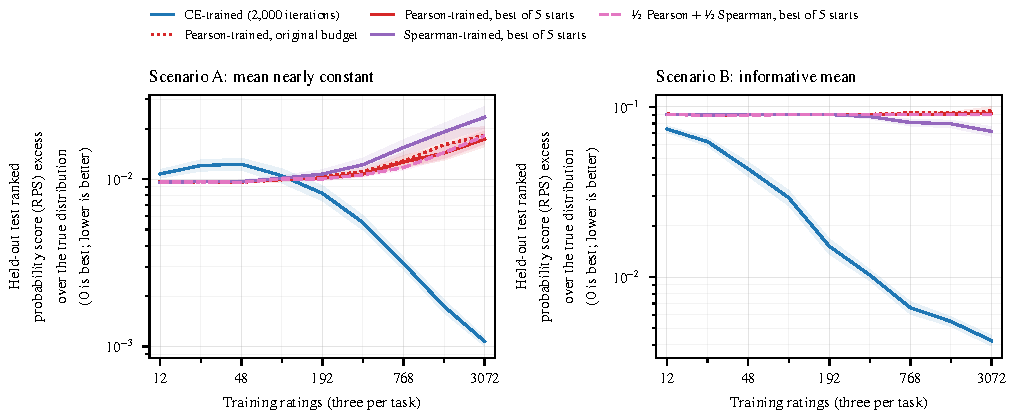
\includegraphics[width=0.96\textwidth]{figures/fig_exp07_restarts.pdf}
\caption{\textbf{Best-of-five restarts with a larger budget improve the correlation fits only slightly, and the CE-trained judge's lead remains.}
Data: synthetic tasks with known distributions (experiment 07), 30 seeds per size, 500 fresh test tasks per seed. Vertical axis: held-out test ranked probability score (RPS) excess over the true distribution (0 is best; lower is better; log scale); horizontal axis: training ratings, three per task.
Every curve has a 95\% percentile bootstrap band over seeds. Solid red and the solid Spearman-trained curve: the best of five starts (the original start and four random ones), each with 2{,}000 L-BFGS-B iterations and 4{,}000 function evaluations, chosen by the penalized training objective; dashed: the same for the half-and-half Pearson and Spearman objective. Dotted red: the original single Pearson start with 400 iterations. Solid blue: the CE-trained judge with one long start.
The CE objective is convex; the correlation objectives are not, and no global optimum was certified.
Bootstrap: 10{,}000 draws.}
\label{fig:exp07}
\end{figure}

\paragraph{The correlation fits rarely converge.}
From 32 training tasks on, the original-budget Pearson fits never converge, and 91\% of the long Pearson fits still hit the 2{,}000-iteration budget.
The half-and-half fits behave the same way (1\% converge at the original budget, and 89\% of the long fits hit the budget), and Spearman fits converge in 28\% at the original budget with 51\% of the long fits hitting it.
The CE-trained, RPS-trained and calibrated-head fits converge in 100\% of fits, and Kendall in 98\%.

\paragraph{Restarts improve the training objective, and the held-out RPS crossovers stay where they were.}
The best of five starts lowers the penalized training objective by more than $10^{-6}$ relative to the first long fit in 57\% to 90\% of the correlation fits (three objectives, nine sizes).
Yet at 1{,}024 tasks the RPS excess of the Pearson-trained judge barely moves. It goes from 0.0183 to 0.0173 in scenario A (CE-trained: 0.0011) and from 0.0949 to 0.0918 in scenario B (CE-trained: 0.0042).
Every crossover on held-out RPS excess is unchanged: 64 tasks (192 ratings) in A for Pearson, Spearman and the half-and-half mix, and 4 tasks (12 ratings) in B.
On held-out CE, only two scenario-A crossovers move, each by one grid step: the Spearman-trained judge's from 32 to 64 tasks and the Kendall-trained judge's from 32 to 16 tasks.
These checks test the optimizer budget and the start; they do not certify a global optimum for any correlation objective.

\paragraph{Numerical check of the cross-entropy gradient.}
A post-hoc review found that the frozen CE function of experiment 13 clips and renormalizes probabilities at $10^{-6}$ and returns an inconsistent gradient when clipping is active.
Refitting every CE judge with the exact objective and gradient leaves the reported results unchanged: in experiment 13 none of 2{,}200 rows differs by more than $10^{-9}$ in any metric, and in experiment 08 none of 4{,}400 fixed-ridge CE rows differs.
Of 4{,}400 validation-tuned CE rows in experiment 08, 338 move, by at most 0.00023 in RPS excess, and one ridge choice changes (the share choosing $c=0.01$ in scenario C at 256 tasks moves from 69\% to 68\%); all 95{,}291 exact-CE fits converged.
The saved Pearson rows came from another machine, which is a separate matter.
Rerunning the frozen code on the review machine reproduces the saved CE and RPS rows (none of 2{,}200 differs).
It does not reproduce the Pearson rows (2{,}198 of 2{,}200 differ, by up to 0.0082 in one row's RPS excess) or the calibrated heads fitted on them (2{,}198 differ, by up to 0.40).
We therefore treat each Pearson-trained curve as one realization of this optimizer and rely on the budget and restart checks above.

\subsection{Where the target's information lies matters more than its complexity (experiment 08)}
\label{app:controlled-complexity}

We fixed the hypothesis and the decision rule of experiment 08 before measuring.
The conjecture (ours, 11-13-2026) was that with little rating data a correlation-trained judge might work better, because it only has to get the mean right, so the number of ratings a CE-trained judge needs should grow with the complexity of the target.
Experiment 08 adds two scenarios with varying means and constant concentration: scenario C has the nonlinear mean of B with $\kappa=e^{1.5}$, and scenario D has the linear mean $\mu=0.5+0.35x$ with $\kappa=e^{1.5}$, the case most favorable to correlation.
Their variances still depend on the mean.
Every judge is experiment 13's softmax-linear model with the same optimizer.
The ridge weight is either fixed at $c=1$ or chosen from $\{0.01,0.1,1,10,100\}$ by four-fold cross-validation over the training tasks.
Cross-validation uses validation RPS for the CE-trained and RPS-trained judges, and validation Pearson correlation (or, as a further variant, validation RPS) for the tuned Pearson-trained judge.
A constant forecast of the training histogram serves as the baseline.
We use 100 seeds, 4 to 2{,}048 training tasks with three ratings each, and 500 fresh test tasks per seed.

\begin{table}[t]
\caption{\textbf{Correlation training wins at low data only in scenario A, where the mean says little; in B, C and D the cross-entropy (CE)-trained judge wins from 12 ratings.}
Experiment 08, held-out test ranked probability score (RPS) excess (0 is best; lower is better) on 500 fresh tasks per seed, 100 seeds.
First column of results: training ratings at which the Pearson-trained judge (fixed ridge) is significantly better than the CE-trained judge (paired 95\% bootstrap interval of the difference of test RPS excess entirely below 0).
Second: the smallest size from which the CE-trained judge (fixed ridge) is significantly better at every larger size.
Third: the same comparison between the validation-tuned CE-trained judge and the validation-tuned Pearson-trained judge.
Ratings are three per task.
We chose each judge by L-BFGS-B (at most 400 iterations) from the training-histogram start; the Pearson objective is not convex, so its results reflect this optimizer, start and budget.}
\label{tab:exp08}
\centering\small
\begin{tabular}{@{}p{0.27\columnwidth}p{0.17\columnwidth}p{0.17\columnwidth}p{0.17\columnwidth}@{}}
\toprule
Scenario & Pearson-trained better at & CE-trained better from & Tuned CE better from \\
\midrule
A: mean nearly constant, spread varies & 12 to 96 ratings & 192 ratings & 96 ratings \\
B: informative mean, spread varies & never & 12 ratings & 12 ratings \\
C: nonlinear mean, constant concentration & never & 12 ratings & 12 ratings \\
D: linear mean, constant concentration & never & 12 ratings & 48 ratings \\
\bottomrule
\end{tabular}

\end{table}

Neither hypothesis holds as stated (\Cref{tab:exp08}; \Cref{fig:ratings-needed} plots the four curves).
The low-data edge of correlation training appears only in scenario A, up to 96 ratings, and not in C or D, where the conjecture predicted it most strongly; the CE-trained judge needs the same 12 ratings in B, C and D.
On held-out correlation, the Pearson-trained judge (fixed ridge) overtakes the CE-trained judge only with plenty of data: from 512 tasks (1{,}536 ratings) in B and C and from 1{,}024 tasks (3{,}072 ratings) in D, and never in A.
Validation tuning is noisy with few tasks. Tuning both judges' ridge moves the crossover of scenario A from 64 to 32 tasks. The tuned CE-trained judge is significantly worse than the fixed-ridge Pearson-trained judge at 4, 8 and 16 tasks in A and at 4 tasks in D.
The Pearson-trained judge ends up worse than the constant forecast.
Its test RPS excess is significantly higher at every tested size from 128 tasks in A, 8 in B, 16 in C and 256 in D (paired 95\% lower bound above 0), and at 2{,}048 tasks the paired differences are +0.016, +0.028, +0.025 and +0.007.
Its held-out Pearson correlation with the true mean reaches 0.85, 0.99, 0.99 and 0.98.

What survives of the conjecture is narrow.
When the target's structure lies in higher moments and the mean carries little signal, a judge that matches the mean and keeps the average spread does well in small samples, and scenario A is consistent with that explanation, which we did not test directly.
What fails: in B, C and D the CE-trained judge has lower test RPS from the smallest tested size.
The ratings needed therefore depend on \emph{where} the target's information lies, not on its complexity alone: scenario B has A's varying disagreement plus an informative mean, and it crosses at 12 ratings.
Which scenario human ratings resemble is open.
On the human-rating sets of experiment 28 the Pearson fit has lower held-out RPS than the CE fit, by a simultaneous one-sided 97.5\% bound, in 19 of 325 cells: 18 at 10 ratings with five per item and one at 4 ratings with one per item (Section~\ref{sec:frozen}).
We did not test small-sample gains for correlation on other human ratings.

\subsection{Why correlation is the wrong primary metric}
\label{app:controlled-metric}

We give four reasons to report a proper score first and correlation second.
\begin{enumerate}
\item \textbf{Even on correlation, training on correlation buys little.} Below 128 training tasks no correlation-trained judge has a higher mean held-out correlation than the CE-trained judge, by the correlation reported for it (Pearson for the Pearson-trained and half-and-half judges, Spearman for the Spearman-trained and Kendall-trained judges), and in scenario A none does at any tested size. The correlation-trained judges overtake only with plenty of data in scenario B (\appref{app:controlled-rank}), while their rating distributions stay far worse (\Cref{fig:exp06-rank}).
\item \textbf{Correlation cannot see what matters.} Maximizing Pearson correlation minimizes the squared error between z-scored judge ratings and z-scored human ratings, so any shift or positive rescaling of the judge's ratings leaves it unchanged; these are exactly the bias and scale terms of squared error (\appref{app:moments-squared}). Any increasing transform leaves Spearman correlation unchanged. Both see one number per item, the mean, so neither identifies scale, signed bias or the pattern of rater disagreement. Correlation ties five different distributions in every replication of experiment 01. In experiment 00 (one seed, 2{,}000 synthetic human scores uniform on 0 to 5), a squashed judge that outputs only 4 or 5 has Pearson correlation 0.877 and Spearman correlation 0.878, against 0.900 and 0.900 for a noisy faithful judge. Its KL divergence to the human marginal histogram (Laplace-smoothed) is 3.420 nats, against 0.001 for the noisy faithful judge.
\item \textbf{Correlation is not a proper scoring rule.} It does not reward reporting the true rating distribution. Its value also depends on how spread out the test items are, not only on the judge, so one cannot average it item by item or compare it across test sets.
\item \textbf{What correlation is still good for.} If the only use is ranking items, Spearman correlation is a reasonable secondary diagnostic. To choose or train a judge that must reproduce human ratings, use a proper loss such as RPS and report correlations alongside it.
\end{enumerate}

\subsection{Retrospective comparison on theorem ratings}
\label{app:controlled-forest}

\Cref{fig:forest} summarizes the matched comparisons on the 75 theorem artifacts (25 tasks, 19 families, 195 expert ratings).
All of the studies reuse these ratings, so they are one body of evidence and not independent replications, and ``held out'' means held out from the fit, not from earlier judge selection.
For mixtures over five frontier judges no difference is established (experiment 02: $+0.0046$, 95\% interval $[-0.0100,+0.0356]$; archived experiment 12: $+0.0056$, $[-0.0059,+0.0181]$).
For the pool of 39 open-weight judges and the combined pool of 44 judges the CE-trained mixture is better ($+0.0502$, $[+0.0238,+0.0754]$; $+0.0405$, $[+0.0237,+0.0575]$).
The best single judge reverses the sign for the 44-judge pool, where selection by Pearson correlation is better ($-0.0317$, $[-0.0638,-0.0047]$), while selection by CE is better for the 39 open-weight judges ($+0.0529$, $[+0.0137,+0.0911]$), and no difference is established for the five frontier judges ($-0.0254$, $[-0.0570,+0.0005]$).
Each entry is the test RPS of the Pearson-trained judge minus that of the CE-trained judge; positive means the CE-trained judge is better.

\begin{figure}[t]
\centering
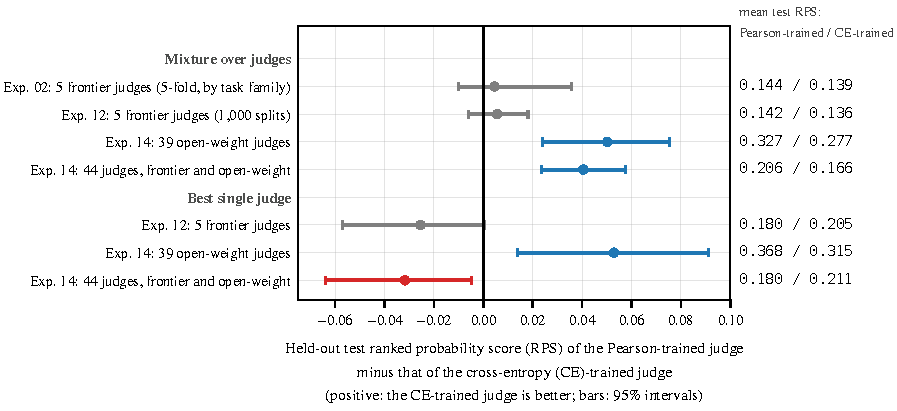
\includegraphics[width=0.82\textwidth]{figures/fig_forest.pdf}
\caption{\textbf{On the 75 retrospective theorem artifacts, the CE-trained mixture is better only for the larger judge pools, and selecting a single judge by Pearson correlation is better for the 44-judge pool.}
Data: held-out test artifacts from 25 tasks and 195 expert ratings, all used in earlier studies, so the comparison is retrospective and not a fresh test set.
Archived experiments 12 and 14 use 1{,}000 random splits with 20 training and 5 test tasks; experiment 02 uses five-fold task-family splits repeated over five partitions.
Horizontal axis: held-out test ranked probability score (RPS) of the Pearson-trained judge minus held-out test RPS of the CE-trained judge (0 means no difference; positive means the CE-trained judge is better; RPS ranges from 0 to 1 and lower is better).
Right column: mean test RPS of the Pearson-trained and the CE-trained judge.
Dots: mean differences; bars: 95\% percentile bootstrap intervals (10{,}000 draws over 25 tasks for archived experiments 12 and 14; 1{,}000 attempted task-family draws with refitting for experiment 02, of which 998 were usable).
Blue: CE-trained judge better; red: Pearson-trained judge better; gray: the interval includes 0.
Mixture weights over the base judges' rating histograms were fitted on the training tasks by an exact Pearson solver or by a convex CE solver with a suboptimality certificate, and single judges by exhaustive search over the pool (\appref{app:protocols}).}
\label{fig:forest}
\end{figure}
